本研究の目的は, 配信に途中参加したユーザがダイジェスト視聴可能なP2Pライブストリーミングシステムを提案することである. この目的を達成するために2つの段階を考える. 1つ目の段階として, まずP2Pネットワーク内でダイジェストを生成することを考える. 動画コンテンツであったり, ライブ映像であっても, ダイジェストを生成するための専用の計算機やサーバを用意することが出来れば, 既存のダイジェスト生成方式を使える. しかし, 本研究ではP2Pライブストリーミングにおいてダイジェストを生成することを考えるため既存の手法は使えない. そこで, P2Pライブストリーミングに特化したダイジェスト生成方式を提案する. 2つ目の段階として, P2Pネットワーク内で作成したダイジェストを保持し, 広めるためのトポロジ設計を行う. システムはP2Pなのでダイジェストを管理する特別なサーバを用意することが出来ない. よって作成したダイジェストはサーバではなく各ピアが管理する. そのため各ピアが役割を持ったトポロジを設計する.

まず最初に\ref{sec:pro-digest}節でダイジェスト生成方式についての提案方式を述べ, 続く\ref{sec:pro-topology}節でトポロジ設計についての提案方式を述べる.

\newpage

\section{ダイジェスト生成方式}\label{sec:pro-digest}
P2Pライブストリーミングを行う際に, 特別なサーバに頼ること無く参加している各ピアがダイジェストを生成出来るような方式を提案する. 本研究では3つの異なる手法に基づいたダイジェスト生成方式を提案する. 1つ目は「増減率に基づくダイジェスト生成方式」(\ref{subsec:pro-sikiiti}節), 2つ目は「前後比較に基づくダイジェスト生成方式」(\ref{subsec:pro-zengo}節), 3つ目は「最小二乗法に基づくダイジェスト生成方式」(\ref{subsec:pro-jijo}節)である.

\subsection{ダイジェスト生成におけるユーザとコメント}
本研究ではある特定の種類, 例えばスポーツなどの映像に特化したダイジェスト生成方式ではなく, どのような種類の映像にも適応可能な汎用的なダイジェスト生成方式を目指す. そのため, 本研究ではP2Pライブストリーミングシステムに参加しているユーザとそのコメント数に着目した. 提案するP2Pライブストリーミングシステムでは, 参加ユーザが配信内容に対して自由にコメント投稿が出来ることを想定する. コメントは1ユーザにつき何回でも投稿出来るものとし, 各ユーザが投稿したコメント数はシステム内で管理しているものとする.

ダイジェスト生成においては単位時間当たりにコメントしたユーザ数を利用する. ユーザ数は1つのコンテンツを視聴しているユーザの数を意味する. ユーザ数はどの種類の映像のコンテンツであっても共通の指標として利用できるため, 汎用的なダイジェスト生成方式を目指すシステムに適している. ユーザ数はコンテンツの継続時間によって増減し, 特定の時刻のユーザ数が多いほど注目度が高いことを意味する. その注目度の高い特定の時刻のコンテンツの内容をダイジェストとして利用することを考える. 継続時間によって変化するユーザ数を用いて, 例えばユーザ数増減グラフ(図\ref{fig:zogen})を作成することが出来る. 提案する3つの方式では, ユーザ数増減グラフにおいて突出している部分「突出点」を発見することによりダイジェストを作成する.

\newpage

\begin{figure}[h]
  \centering
  \includegraphics[width=1\hsize]{fig/zogen.eps}
  \caption{あるコンテンツのユーザ数増減グラフ}
  \label{fig:zogen}
\end{figure}

ダイジェスト生成方式を提案するにあたり, 達成すべき要求条件を以下にあげる.

\begin{itemize}
\item 特定の種類のコンテンツに依存しないダイジェスト生成方式であること
\item P2Pライブストリーミングに特化したダイジェスト生成方式であること
\item 生成されたダイジェストの映像によってコンテンツの内容の全体把握が出来ること
\end{itemize}

\subsection{増減率に基づくダイジェスト生成方式}\label{subsec:pro-sikiiti}
1つ目は「増減率に基づくダイジェスト生成方式」である. これはユーザ数が増加している時を始点, ユーザ数が減少している時を終点とし, 始点から終点までで最もユーザ数の多い点を「突出点」として抽出する方式である. ユーザ数の増加率と減少率をそれぞれ閾値として決定する. 増加率を超えた時の値を始点とし, その後減少率を超えた値が出現するまで探してその値を終点とする.  これは以下の式\ref{siki:sikiiti}に従う.

\begin{eqnarray}
始点: \frac{X_{t+T}-X_{t}}{X_{t}} \geq Th_{inc} \nonumber \\
終点: \frac{X_{t+T}-X_{t}}{X_{t}} \leq Th_{dec} \nonumber \\
なお, X_{t}は始点または終点となる. \nonumber \\
(X_{t}は時刻tにおけるユーザ数,Tは一定期間, Th_{inc}とTh_{dec}は閾値)&&
\label{siki:sikiiti}
\end{eqnarray}


図\ref{fig:sikiiti}は増減率に基づくダイジェスト生成方式を適用したグラフである. 縦に赤い線が始点であり, 縦に青い線が終点である. 始点は数分間のユーザ数の増加率を計算したのち, その増加率が閾値を超えた点を示している. 終点は数分間のユーザ数の減少率を計算したのち, その減少率が閾値を超えた点を示している. 縦に緑の線は「突出点」を示しており, この部分をダイジェストとして抽出する.

\begin{figure}[h]
  \centering
  \includegraphics[width=1\hsize]{fig/sikiiti.eps}
  \caption{増減率に基づくダイジェスト生成方式を適用したグラフ}
  \label{fig:sikiiti}
\end{figure}

\subsection{前後比較に基づくダイジェスト生成方式}\label{subsec:pro-zengo}
2つ目は「前後比較に基づくダイジェスト生成方式」である. これは, ある点についてユーザ数が前後で増加かつ減少している場合を「突出点」として抽出する方式である. この方式も1つ目の方式と同様にユーザ数の増加率と減少率をそれぞれ閾値として決定し, それぞれの値を超えた場合に「突出点」を決定する. これは以下の式\ref{siki:zengo}に従う.

\begin{eqnarray}
  \frac{X_{t}-X_{t-T}}{X_{t}} \geq Th_{inc} \wedge \frac{X_{t+T}-X_{t}}{X_{t}} \geq Th_{dec} \Rightarrow X_{t}は突出点 \nonumber \\
  \frac{X_{t}-X_{t-T}}{X_{t}} \geq Th_{inc} \wedge \frac{X_{t+T}-X_{t}}{X_{t}} \geq Th_{dec} \Rightarrow X_{t}は突出点 \nonumber \\
  (X_{t}は時刻tにおけるユーザ数, Tは一定期間, Th_{inc}とTh_{dec}は閾値) &&
  \label{siki:zengo}
\end{eqnarray}

図\ref{fig:zengo}は前後比較に基づくダイジェスト生成方式を適用したグラフである. 縦に緑の線は「突出点」を示しており, この部分をダイジェストとして抽出する. 1つ目の方式との違いは, 先に「突出点」となる候補を探し, その点が正しい「突出点」であるかを前後の増減率を計算して決定している点である.

\begin{figure}[h]
  \centering
  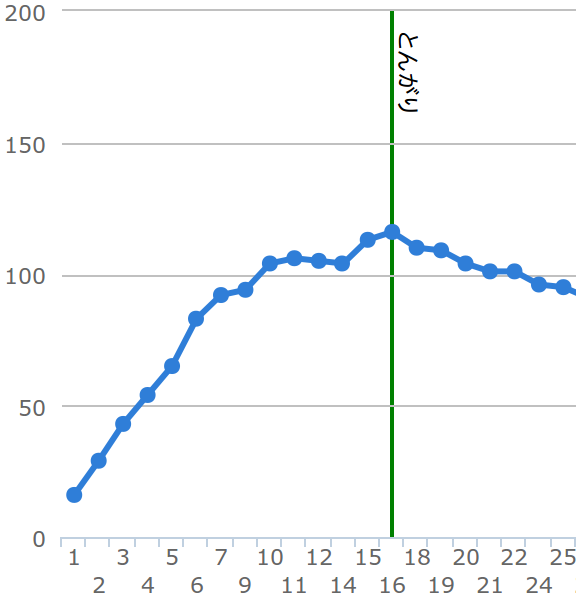
\includegraphics[width=1\hsize]{fig/zengo.eps}
  \caption{前後比較に基づくダイジェスト生成方式を適用したグラフ}
  \label{fig:zengo}
\end{figure}

\newpage

\subsection{最小二乗法に基づくダイジェスト生成方式}\label{subsec:pro-jijo}
3つ目は「最小二乗法に基づくダイジェスト生成方式」である. これは, ユーザ数増減グラフに数点間の最小二乗法を適用し, それによって近似された2直線の重なりが鋭角な点を「突出点」とし抽出する方式である. 最小二乗法を適用した際の直線の重なりの角度を閾値として決定し, その値を超えた場合にその点を「突出点」として決定する. これは以下の式\ref{siki:jijo}に従う.

\begin{eqnarray}
  \arctan \left(\frac{slope_{line2} - slope_{line1}}{1+slope_{line2}*slope_{line1}}\right) \leq Th_{Angle} \nonumber \\
  \Rightarrow 直線の重なり部分が突出点 \nonumber \\
  (slope_{line1}およびslope_{line2}は直線の傾き, Th_{Angle}は閾値) &&
  \label{siki:jijo}
\end{eqnarray}

図\ref{fig:jijo}は最小二乗法に基づくダイジェスト生成方式を適用したグラフである. 点と点の間のカラフルな線が最小二乗法を適用した時の直線であり, 縦に緑の線が「突出点」を示しており, この部分をダイジェストとして抽出する.

\begin{figure}[h]
  \centering
  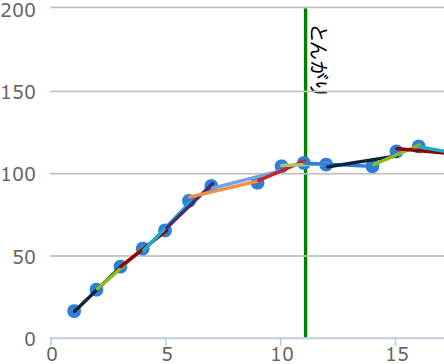
\includegraphics[width=1\hsize]{fig/jijo.eps}
  \caption{最小二乗法に基づくダイジェスト生成方式を適用したグラフ}
  \label{fig:jijo}
\end{figure}

\newpage

\subsection{既存のダイジェスト生成方式との比較}
関連研究であげた既存のダイジェスト生成方式との比較の結果を表\ref{tbl:compare-digest}に示す. 橋本らの提案したスポーツ映像を対象とした方式を「方式1」, 熊野らの提案した野球の実況中継映像を対象とした方式を「方式2」, 本研究で提案する方式を「提案方式」とする.

\begin{table}[h]
  \caption{既存のダイジェスト生成方式との比較}
  \label{tbl:compare-digest}
  \centering
      {\small
        \begin{tabular}{|l|l|l|l|}
          \hline
          & 方式1 & 方式2 & 提案方式 \\ \hline \hline
          リアルタイム性 & 対応していない & 対応している & 対応している \\ \hline
          P2Pへの対応 & 対応していない & 対応していない & 対応している \\ \hline
          汎用性 & スポーツに特化 & 野球に特化 & 様々な種類に適用可能 \\ \hline
        \end{tabular}
      }
\end{table}

方式1や方式2に比べ, 提案方式ではP2Pライブストリーミングにおいて汎用的なダイジェスト生成方式であることがわかる.

なお, 本節で提案した3つの方式は\ref{sec:ev-digest}節にて具体的なスレッショルド値等を与え, その優劣を評価する.

\newpage

\section{トポロジ設計}\label{sec:pro-topology}
これまでは, P2Pライブストリーミングにおいて汎用的なダイジェスト生成方式について述べてきた. ここでは生成されたダイジェストをP2Pネットワーク内で保持し, それを配信するためのトポロジ設計を提案する.

トポロジの構成としては主にツリー構造とメッシュ構造が存在する. ツリー構造とは, 1つのノードが複数の子を持ち, 1つの子が複数の孫を持つという形になっており, 枝分かれをしながら階層が深くなっていく構造のことである. 木が幹から枝に, 枝から葉に分かれていく様子に似ていることからツリー構造と言われている. ツリー構造は構造が単純なため構築が容易であるが, その反面1つのノードが居なくなるとそれより下の子全員が切り離されてしまうので耐故障性に弱いという特徴がある. メッシュ構造とはツリー構造のように親と子のみと接続するのではなく, 複数のノードが接続し相互に通信を行う構造のことである. 複数のノードが接続しているので網の目(mesh)のように見えるためメッシュ構造と言われている. メッシュ構造はツリー構造のように特定のノードからのみ受信するのではなく, 複数のノードから受信できるので耐故障性に優れている. しかし必然的に各ノードの接続数が増え, 複数経路を通るため遅延が大きくなってしまうという問題がある. これらの問題を解決する構造として, 関連研究で紹介した複数クラスタ型が登場した. 複数クラスタ型はツリー構造のように中継ノードにストリームを渡し, 各中継ノードはそれぞれクラスタを作成してクラスタの中ではメッシュ構造のように複数のノード同士が接続している構造である. 複数クラスタはツリー構造とメッシュ構造の欠点を補っている. 本研究では複数クラスタ型のトポロジ設計にする.

複数クラスタ型では中継ノードを選ぶ必要がある. また, 本研究ではP2Pのライブストリーミングシステムを対象としているため, ダイジェストを管理するためのサーバを用意することが出来ない. そのため, 生成されたダイジェストは特定のノードに管理させることにする. さらに, 中継ノードへの負担を軽減するためにクラスタ内へストリームを広めるためのノードも必要である. このように, 各ノードに役割を持たせたトポロジ設計にする. 以下では, 中継ノードを「ゲートノード」, ダイジェストを管理をするノードを「ダイジェストノード」, クラスタ内へストリームを広めるためのノードを「セミゲートノード」と呼ぶこととする.

トポロジを提案するにあたり, 達成すべき要求条件を以下にあげる.

\begin{itemize}
\item ライブストリーミングの映像を見られるだけの性能があること
\item 少ない遅延でパケットが届くこと
\item ダイジェストをP2Pネットワーク内に確保できること
\end{itemize}

\subsection{トポロジ設計におけるユーザとコメント}
ダイジェスト生成においては単位時間当たりにコメントしたユーザ数を利用した. トポロジ設計においてもユーザ数とそのコメント数を利用する. あるコンテンツを視聴しているユーザのコメント数が多いということは, そのユーザが, 視聴しているコンテンツに対してアクティブであり, 配信から離脱する可能性が低いことを意味する. このような離脱可能性の低いノードを中継ノードである「ゲートノード」や, ダイジェストを管理する役割を担う「ダイジェストノード」に適用する.

ダイジェスト生成で紹介した図\ref{fig:zogen}は, 単位時間当たりにコメントしたユーザ数の増減グラフを表している. このグラフの値に1ユーザ当たりのコメント数を付与すると例えば以下のような表\ref{tbl:user-comment}が出来上がる.

\begin{table}[h]
  \caption{単位時間における各ユーザ毎のコメント判別グラフの例}
  \label{tbl:user-comment}
  \centering
      {\small
        \begin{tabular}{|c||c|c|c|c|c|} \hline
          & \multicolumn{4}{|c|}{時刻(ms)} & 合計(ユーザ毎のコメント数) \\ \hline \hline
          ユーザ & 0 & 1 & 2 & $\cdots$ & \\ \hline \hline
          ユーザ1 & ○ & ○ & × & $\cdots$ & 15 \\ \hline
          ユーザ2 & ○ & ○ & ○ & $\cdots$ & 5 \\ \hline
          ユーザ3 & × & × & × & $\cdots$ & 8 \\ \hline
          $\vdots$ & $\vdots$ & $\vdots$ & $\vdots$ & &  \\ \hline
          合計(時刻におけるコメントしたユーザ数) & 4 & 6 & 10 & &  \\ \hline
        \end{tabular}
      }
\end{table}

この表は単位時間における各ユーザ毎のコメント判別グラフの例である. コメントをした場合は○, コメントをしなかった場合は×が書かれている. この表において, n番目の時間コメントしたユーザ数の合計をグラフにすると図\ref{fig:zogen}が出来上がる. ユーザ毎のコメント数の合計を見ると以下の図\ref{fig:comment}のようになる. 図\ref{fig:comment}は各コメント数におけるユーザ数の割合を示しており, 離脱可能性の高いノードや, 逆に低いノードの割合を知ることが出来る. 各ノードに役割を割り当てる際に, このグラフを利用する.

\begin{figure}[h]
  \centering
  \includegraphics[width=1\hsize]{fig/comment.eps}
  \caption{各コメント数におけるユーザ数}
  \label{fig:comment}
\end{figure}

\newpage

\subsection{ノードの役割}
各ノードにはそれぞれ役割を割り当てる. 役割は「ゲートノード」, 「セミゲートノード」, 「ダイジェストノード」, 「その他のノード」に分けられる. それぞれについて解説していく.

\subsubsection{ゲートノード}
配信者ノードから配信されたコンテンツのパケットをクラスタ内で一番最初に取得する. また, 他のクラスタのゲートノードと繋ぎコンテンツのパケットを送受信する役割を担う.

\subsubsection{セミゲートノード}
クラスタ内でゲートノードから受信したパケットをクラスタ内部に拡散する役割を担う.

\subsubsection{ダイジェストノード}
ダイジェストの作成を行う, また作成したダイジェストを保有し, 新規参加ノードへ送信する役割を担う.

\subsubsection{その他のノード}
その他のノードに, トラッカーサーバとノーマルノードが存在する. トラッカーサーバは全ノードのコメント数, 帯域幅, ホップ数を常に計算する. トラッカーサーバには全てのノードが接続し, 全てのノードの情報を管理する.

ノーマルノードはどの役割にも属さないノードのことである. ノーマルノードの中にはダイジェストを取得し終えたノードと, 新規参加したばかりでまだダイジェストを取得し終えていないノードが存在する.

\subsection{ノードの役割決定方法}
ノードの役割を決定する方法について述べる. 図\ref{fig:role}に図解したものを載せる.

各ノードは固有の帯域幅, コメント数を持っており, この値を元に役割を決定する.

ノードの役割は, ダイジェストノード, ゲートノード, セミゲートノード, ノーマルノードの順番で決定する. まず, 各ノードをコメント数の降順に並び替える. 並び替えたノードのうち, 上位のいくつかのノードをダイジェストノードとして選出する. 残ったノードのうちゲートノードとセミゲートノードの分のノードを取り出し, 帯域幅の降順に並び替える. 並び替えたノードのうち, 上位いくつかのノードをゲートノードとして選出する. さらにそのゲートノードを除いた上位いくつかのノードをセミゲートノードとして選出する. ゲートノードとセミゲートノードは同じ数だけ選出する. 残りのノードをノーマルノードとする.

\begin{figure}[h]
  \centering
  \includegraphics[width=1\hsize]{fig/role.eps}
  \caption{ノードの役割を決定する方法}
  \label{fig:role}
\end{figure}

\newpage

\subsection{ノード間の接続方法}
図\ref{fig:topology}は提案システムのトポロジの様子である. 2つのクラスタがあり, その外側の接続と, クラスタ内の接続について示している.

まず, クラスタ外部間での接続方法を示す. 配信者ノードは全てのゲートノードと接続する. 1つのゲートノードは他のクラスタのゲートノード1つずつと接続する.

次にクラスタ内部での接続方法を示す. 1つのゲートノードは他の全てのゲートノードと接続する. また, 全てのゲートノードは1対1の関係となるセミゲートノードが存在し, 1つのゲートノードはその対応するセミゲートノード1つずつと接続する. 1つのセミゲートノードはいくつかのダイジェストノードと接続する. またノーマルノードいくつかと接続する. 1つのダイジェストノードはダイジェスト未取得ノーマルノード全てと接続する. ノーマルノードは他のノーマルノードのいくつかと接続する.

\begin{figure}[h]
  \centering
  \includegraphics[width=1\hsize]{fig/topology.eps}
  \caption{提案システムのトポロジ}
  \label{fig:topology}
\end{figure}

\newpage

\subsection{新規参加ノードについて}
新規ノードの参加手順について述べる. 図\ref{fig:seq}は新規ノードの参加手順を示したシーケンス図である.

新規参加ノードはネットワーク接続時に配信者ノードにつなぐ. その後, 配信者ノードはトラッカーサーバへ新規参加ノードの存在を伝える. トラッカーサーバは配信者ノードから受け取った新規参加ノードの情報を元に, 帯域や各クラスタへの論理ホップ数を計算し, 最も論理ホップ数の小さいクラスタに配置される. 新規参加ノードはクラスタに配置された後, クラスタ内のダイジェストノードからダイジェストを受け取り, ダイジェストを視聴する.

\begin{figure}[h]
  \centering
  \includegraphics[width=1\hsize]{fig/seq.eps}
  \caption{新規ノードの参加手順シーケンス図}
  \label{fig:seq}
\end{figure}

\newpage

\subsection{再構築のタイミング}
再構築のタイミングは3つ存在する. 1つ目は新規参加ノードがダイジェストを取得し終わった時である. ダイジェストノードとの接続を切断したあと, 帯域に応じて接続数を決定する. 帯域が十分に高い場合にはセミゲートノードになる. 2つ目はノーマルノードのコメント数が一定数を超えた時である. この場合, 対象のノードはコメント数が多く, 離脱可能性が低いノードであると判断される. そしてその対象のノードはダイジェストノードになり, ダイジェストを保有し, 管理する役割を担う. 3つ目はノードが離脱した時である. この場合には, 離脱ノードに接続していたノードは接続数を維持するように他のノードと再接続する. 特にゲートノードが離脱した場合にはセミゲートノードが即座にゲートノードになる. また, 特にセミゲートノードが離脱した場合には, クラスタの中で最も帯域が高いノードがセミゲートノードになる.

\newpage

\subsection{既存のトポロジ設計との比較}
関連研究であげた既存のトポロジ設計との比較の結果を表\ref{tbl:compare-topology}に示す. 比較する全てのトポロジは複数クラスタ型である. Yang Guoの提案したHCPSを「HCPS」, 元橋らの提案した重畳クラスタ木方式の動画配信システムを「重畳型」, Huey-Ing Liuらの提案したMeTreeを「MeTree」, 本研究で提案する方式を「提案方式」とする.

\begin{table}[h]
  \caption{既存のトポロジ設計との比較}
  \label{tbl:compare-topology}
  \centering
      {\small
        \begin{tabular}{|c|c|c|c|c|} \hline
          & HCPS & 重畳 & MeTree & 提案 \\ \hline \hline
          ダイジェスト & なし & なし & なし & あり \\ \hline
          クラスタ & 完全結合 & 一部メッシュ & 一部メッシュ  & 一部メッシュ \\
          \hline
          ゲートノード & 高帯域ノード & 滞在時間の長いノード & 高帯域ノード & \shortstack{高帯域+ \\ コメント数の多いノード} \\
          \hline
        \end{tabular}
      }
\end{table}

提案システムは, P2Pのライブストリーミングにおいてダイジェストノードという役割を配置するなど, 生成したダイジェストを保持出来る構造になっている. また, クラスタの中身は一定の接続数を満たしながら遅延の少ないメッシュ構造になっている. さらにゲートノードの選出方法として高帯域のノードを選ぶことはもちろんだが, さらに離脱可能性を考えてコメント数の多いノードを選出している.

